
\subsection{Le test d'écoute Tomatis\textsuperscript \textregistered }
Par cette brève introduction, nous pouvons ainsi mieux percevoir l'importance que Tomatis donnait à l'oreille, donc à l'écoute et à ses recherches pour accompagner le patient dans sa thérapie.
L'harmonie, l'équilibre et le bien-être du patient sont les buts auxquels tendent  toutes thérapies. C'est 
dans ce sens que Tomatis a élaboré sa courbe dite idéale, référence d'équilibre dans son test, dont nous 
allons rapidement brosser l'historique pour amener une meilleure compréhension de cette technique.
%Il convient à présent de se pencher de manière plus spécifique sur
%Tomatis, puisque ce travail repose notamment sur son test d'écoute.
Dans son ouvrage ``Éducation et
    Dyslexie''\autocite {tomatis:education}, la représentation graphique du
 test de capacité d'écoute distingue l'écoute générale de
 l'auto-écoute \autocite {Tomatislangage}, consistant  en un processus
   circulaire entre sa propre  émission vocale et son écoute, inhérent
   à l'apprentissage.
  % ( ``L'oreille et le langage''  (1963), Ed. Seuil,  p.72)
 Apparaissent ainsi les modifications respectives
 de la courbe aérienne et de la courbe osseuse, entraînant une nouvelle vision
 du concept d'écoute \autocite {tomatis_conf}.%\footnote{<<\,Considérations sur le test d'écoute\,>>. 
 %Propos
  %	recueillis au cours du \textsc{iii}\ieme\ congrès international
  	%d'audio-psycho-phonologie (Anvers 1973) lors d'un entretien
       % avec B. Auriol. }
       Tomatis a défini la «courbe d'écoute idéale», celle qui correspond à l'oreille absolue
des chanteurs et des musiciens, en particulier du ténor italien Enrico
Caruso (1873--1921) dont l'analyse vocale a été effectuée à partir de
disques 78 tours. 

\begin{center}
	\begin{figure}[h]
		\centering
		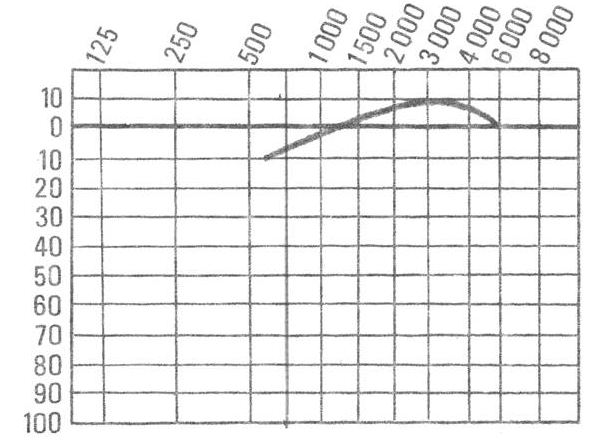
\includegraphics[width=0.7\linewidth]{images/graphiques/courbecarusoideale}	
		\caption{Courbe de Caruso \autocite{Tomatislangage} }
	\end{figure}	
\end{center}
La courbe de Caruso, dite idéale de réponse (Fig. 3.4), a pu être considérée comme
optimale et de référence, caractérisée d'une part par des fréquences allant de 500 et 2000
Hz, par une pente d\textquoteright environ 6 à 18 db/octave,
et d'autre part par un dôme entre 2000 et 4000 Hz.
Le bon fonctionnement de l'oreille a été confirmé par la courbe
de Wegel\footnote{Cf. Annexe \ref{acoustique} p. \pageref{acoustique}}, celle-ci représentant   \enquote 
{les limites fréquentielles graves et 
aigues répondant au seuil 
minimum et maximum (seuil de la douleur) de notre perception auditive } 
\autocite{Tomatislangage}.
 Le travail d'acquisition de ce tracé correspond à l'harmonisation
découlant d'une bonne régulation des deux muscles de l'oreille moyenne
sur la pression interne du
labyrinthe.
Ainsi, l'évaluation finale de ce processus mettra en évidence la différence
d'avec la courbe idéale.
Lorsque le profil des
courbes est continu, parallèle, sans irrégularités et sans
distorsions, on parle d'harmonie, qui règle à son tour
la régulation des émotions, comme on le verra par la suite et conformément à
ce qui avait été annoncé au début de ce travail.
 \\
Etre à même de comprendre la perception du sujet, d'analyser ses blocages, sa problématique, 
n'est pas toujours tâche facile.
%Si, par exemple, à l'issue d'un traitement en musicothérapie, des difficultés subsistent, comme des 
%réactions très fortes à un son précis difficilement explicable, 
 Une distorsion décelée grâce à un test 
de capacité d'écoute peut amener pour le patient comme pour le thérapeute un élément de réponse  et 
corroborer à une 
meilleure  
compréhension au 
processus entrepris.
Une chanteuse diagnostiquée 1° stade de dépression, accompagnée d'une 
détérioration progressive de sa voix, a pris conscience différemment de son état 
par le test d'écoute révélant une distorsion 
importante dans les hautes fréquences. 
%prendre conscience différemment  de sa problématique et contribuer à son rétablissement.
En effet, les détériorations vocales et les troubles de l'humeur peuvent être expliqués parce que la 
capacité d'écoute est perturbée, (Cf. p.18 \autocite{affectiveDisorders}), ce qui change 
considérablement le point de vue.
Autrement dit, les pertes de sa capacité d'écoute sur les hautes fréquences peuvent avoir non seulement 
un lien avec ses difficultés vocales mais aussi avec son état dépressif. Cette mise en résonance est 
source de prise de conscience et mise à distance de la problématique.
%Nous assistons à un renversement de la problématique.
% une grande difficulté  à percevoir les hautes fréquences et donc à les reproduire


 Par définition, la distorsion d'écoute\footnote {Cf. Annexe \ref{acoustique} p. 
 \pageref{acoustique}} 
 %{Cf. 
 %Annexes A. 2. 1}
 est consécutive à une interprétation
erronée des informations transmises entraînant un dysfonctionnement
des deux muscles destinés à favoriser l'arrivée
harmonieuse du son dans l'oreille interne, comme nous l'expliquerons plus en détails ci-après.
En cas d'altération du message sensoriel,
le cerveau déclenche un mécanisme de protection sous forme
d'inhibition de l'écoute, avec le relâchement des deux muscles en
question. 
 \\
Cette faculté d'écoute déjà prête à la naissance peut subir des
altérations avec l'âge et
le temps et affaiblir la protection contre les agressions, raison pour
laquelle la phylogénèse \footnote{ phylogenèse: étym. $>$ grec $\phi
  \upsilon \lambda o \nu $: race; en biologie, le mode de formation des espèces, le développement
  des espèces en cours de l'évolution; tout ce qui (ontogenèse:
  étym. $>$ grec. $\tilde{\omega}\nu$, $o \nu \tau o
  \sigma$: l'être,
ce qui est).}  a intégré la distorsion comme défense
efficace.
B. Auriol nous fait
remarquer que
\enquote {les différents maux (l'otite, l'eczéma, l'hyper
ou hypo sécrétion de sébum) peuvent être compris comme des problèmes physiques liés à l'interaction des sons refusés
inconsciemment} \autocite [19--20]  {auriol:cle}.
Le pouvoir protecteur du cerveau consiste en un  ``étouffement'' de
certaines fréquences, \enquote {en engageant les zones corticales prédestinées
tant à
l'intégration sonore qu' à l'écoute sélective,  avec l'aide synergique de la
modification des impulsions électriques et l'augmentation de
l'irrigation sanguine} \autocite [14] {auriol:cle};
cet ``étouffement'' correspond à la distorsion.
%\autocite {tomatis:education}.
D'ailleurs,  parmi les nombreux apports de Zwicker, nous retenons que 
notre 
système d'écoute peut rendre
attentif ou sourd à certaines fréquences ou à certains patterns
spectraux, mais peut aussi construire des sons fantômes comme dans les --- ``sons de 
Zwicker'' --- (1964) \autocite[p 84] {auriol:cle}.
\\
Ainsi nous disposons de quelques éléments-clés pour la compréhension
sur le phénomène de la ``distorsion audiométrique'' \autocite
{auriol:cle}, sujet déjà abordé en introduction et dont il sera également question dans l'approche
clinique.
\\
%\enquote{\emph{L'oreille a un
%psychisme\autocite[{tomatis:loreille}.}}
